\documentclass{article}

% ------ |
% TITLES |
% ------ |

\usepackage{titlesec}

% CHAPTER STYLING (LINES ABOVE & BELOW, CENTERED, BIG)
\titleformat{\chapter}
	{\titlerule\vspace{0.3\baselineskip}\normalfont\Huge\centering}
  	{\Roman{chapter}. }{0pt}{}[\titlerule]
\titlespacing*{\chapter}{0pt}{0pt}{\baselineskip}

% SECTION STYLING
\titleformat{\section}
 	{\normalfont\bfseries}
	{}{0pt}{}
	\titlespacing*{\section}{0pt}{0.5\baselineskip}{0.5\baselineskip}

% General

\usepackage{multicol} % multicol support
\usepackage{blindtext} % TODO to be removed
\usepackage{amsmath} % math rendering
\usepackage{tikz}

% DIRECTORY PATHS
 }

% metadata

\date{Nov. 2025}
\title{\textbf{Graphenthorie}\\Grundlagen, netzwerktechnische Anwendungen, Fallbeispiele}
\author{Felix Friesenbichler \and Marcel Ogorevc}

\begin{document}

\maketitle

\tableofcontents

\newpage

Graphentheorie bildet die Grundlage für das Verständnis komplexer 
Vernetzungsstrukturen. Ursprünglich aus mathematischen Fragestellungen 
entwickelt, ist sie heute ein zentrales Werkzeug zur Modellierung und Analyse
moderner Informations- und Kommunikationssysteme. Besonders in der Internet -
und Netzwerktechnologie unterstützt sie die Beschreibung von Topologien, 
die Optimierung von Datenwegen sowie die Bewertung von Zuverlässigkeit und 
Effizienz technischer Infrastrukturen.

\section{Grundlagen}

Ein einfacher Graph $G$ besteht aus Knoten und Kanten. Dabei gilt,

\begin{equation}
    G = (V, E)
\end{equation}

wobei $V$ die endliche Menge an Knoten und $E$ die endliche Menge an Kanten 
darstellt. Genauer lässt sich $E$ als 2-elementige Teilmenge von $V$, also 
$E = [V]^2$, beschreiben. Das bedeudet, dass eine Kante $e$ jeweils durch 
zwei Knoten $v_1$ und $v_2$ definiert wird.
  % Einführung

\include{ch2/ch2}  % Entwicklung

\begin{multicols}{2}

\blindtext

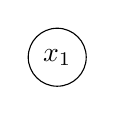
\begin{tikzpicture}[main/.style = {draw, circle}]
	\node[main] (1) {$x_1$};
\end{tikzpicture}

\end{multicols}

\section{Anwendungen \& Fallbeispiele}

\subsection{BGP}
\subsection{OSPF}
\subsection{MPLS}

\section{Ausblick \& Beispielfrage}

\end{document}
